\subsection{Least-Squares Line(最小二乘拟合曲线)}

\frame{
\begin{block}{}
In science and engineering, it is often the case that an experiment produces a set of data points $(x_1, y_1), \ldots, (x_n, y_n)$, where the abscissas $\{ x_k \}$ are distinct. 
\end{block}
\begin{center}
$\Downarrow$
\end{center}
\begin{block}{}
One goal of numerical methods is {\Large to determine a formula $y = f(x)$ that relates these variables. }
\end{block}
\begin{center}
$\Downarrow$
\end{center}
\begin{block}{In this section we emphasize the class of linear functions of the form}
\begin{equation*}
y = f(x) = A x + B
\end{equation*}
\end{block}
}

\frame{
\begin{block}{In the last chapter  we saw how to construct a polynomial that passes through a set of points.}
\begin{itemize} 
\item If all the numerical values $\{ x_d \}$, $\{ y_d \}$ are known to several significant digits of accuracy, then polynomial interpolation can be used successfully; otherwise, it cannot. 
\vspace{5mm}
\item Some experiments are devised using specialized equipment so that the data points will have at least five digits of accuracy. 
\end{itemize}
\end{block}
}

\frame{
\begin{block}{\Huge However, }
\begin{itemize} 
\item  many experiments are done with equipment that is reliable only to three or fewer digits of accuracy. 
\vspace{5mm}
\item  there is an experimental error in the measurements,  and although three digits are recorded for the values $\{ x_d \}$ and $\{ y_d \}$, it is realized that the true value $f(x_k)$ satisfies 
\begin{equation*}
f(x_k) = y_k + e_k
\end{equation*}
where $e_k$ is the measurement error. 
\end{itemize}
\end{block}
}

\frame{
\begin{block}{}
\begin{center}
{\Huge How do we find the best linear approximation of the above form  that goes near (not always through) the points? }
\end{center}
\end{block}
}

\frame{
\begin{block}{To answer this question, we need to discuss the {\Large errors} (also called {\Large deviations} or {\Large residuals}): }
\begin{equation*}
e_k = f(x_k) - y_k \ \ \ \ \ for \ \ 1 \le k \le N
\end{equation*}
\end{block}
\begin{block}{There are several norms that can be used with the residuals in (4.3) to measure how far the curve $y = f(x)$ lies from the data. }
\begin{table}[!h]
\begin{tabular}{l l}
& \\
Maximum error : & $E_{\infty} (f) = max_{1 \le k \le N}  \left\{  \left|  f(x_k)  - y_k \right|  \right\}$ \\
& \\
Average error : &  $E_1 (f) = \frac{1}{N} \sum_{k=1}^{N} \left|   f(x_k)  - y_k \right| $ \\
& \\
Root-mean-square error : &  $E_2 (f) =  \left\{ \frac{1}{N} \sum_{k=1}^{N} \left|   f(x_k)  - y_k \right|^2  \right\} ^{\frac{1}{2}} $
\end{tabular}
\end{table}
\end{block}
}

\frame{
\frametitle{Example}
\begin{block}{Compare the maximum error, average error, and rms error for the linear approximation $y = f (x ) = 8.6 − 1.6x$ to the data points $(−1, 10)$, $(0, 9)$, $(1, 7)$, $(2, 5)$, $(3, 4)$, $(4, 3)$, $(5, 0)$, and $(6, −1)$.}
\begin{columns}
\begin{column}{0.5\textwidth}
\begin{figure}
Table 4.1 Calculations for Finding $E_1( f )$ and $E_2( f )$ for Example 4.1
\begin{center}
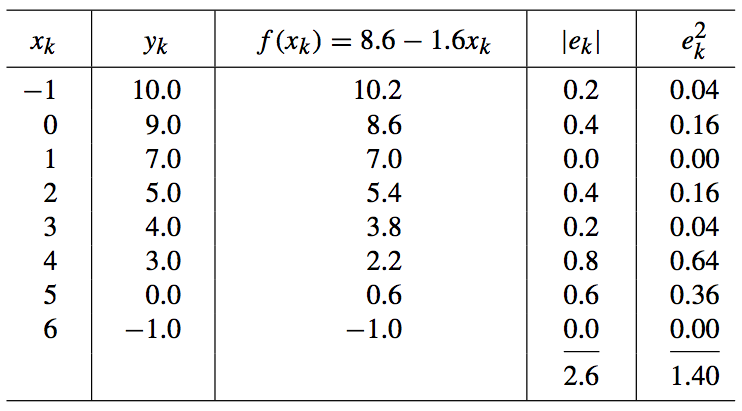
\includegraphics[width=50mm]{chap-4/tab_5-1.png}
\end{center}
\end{figure}
\end{column}
\begin{column}{0.5\textwidth}
\begin{table}[h]
\begin{tabular}{l l}
$E_{\infty} (f)$ & $=  \max \{  0.2, 0.4, 0.0, 0.4,$ \\
&  $ 0.2, 0.8, 0.6, 0.0  \} $ \\
& $= 0.8$ \\
$E_1 (f)$  & $= \frac{1}{8} (2.6) = 0.325 $ \\
& \\
$E_2 (f)$  & $ =  \left( \frac{1.4}{8}  \right) ^{\frac{1}{2}} = 0.41833 $
\end{tabular}
\end{table}
\end{column}
\end{columns}
\end{block}
}

\frame{
\begin{block}{According to Example 4.1}
\begin{itemize}
\item We can see that the maximum error is largest, and if one point is badly in error, its value determines $E_{\infty} (f)$. 
\vspace{0.3cm}
\item The average error $E_1 (f)$ simply averages the absolute value of the error at the various points.  
 It is often used because it is easy to compute. 
\vspace{0.3cm}
\item The error $E_2 (f)$ is often used when the statistical nature of the errors is considered. 
\end{itemize}
\end{block}
\begin{center}
$\Downarrow$
\end{center}
\begin{block}{}
The third norm $E_2(f)$ is the traditional choice because it is much easier to minimize computationally. 
\end{block}
}

\frame{
\frametitle{Finding the Least-Squares Line}
\begin{block}{}
\begin{itemize}
\item Let $\{(x_k,y_k)\}_{k=1}^N $ be a set of $N$ points, where the abscissas $\{ x_k\}$ are distinct. 
\item The {\Large least-squares line} $y = f(x) = Ax + B$ is the line that minimizes the root-meansquare error $E_2 (f)$. 
\end{itemize}
\end{block}
\begin{itemize}
\item The quantity $E_2(f)$ will be a minimum if and only if the quantity $N(E_2(f))^2 = \sum_{k=1}^N (Ax_k + B - y_k)^2$ is a minimum. 
\item The latter is visualized geometrically by minimizing the sum of the squares of the vertical distances from the points to the line. 
%\item The next result explains this process.
\end{itemize}
}

\frame{
\begin{block}{ Theorem (Least-Squares Line).}
Suppose that $\{ (x_k , y_k )\}_{k=1}^N$ are $N$ points,  where $k=1$ the abscissas $\{ x_k \}_{k=1}^N$ are distinct. 
The coefficients of the least-squares line
\begin{equation*}
y = Ax + B 
\end{equation*}
are the solution to the following linear system, known as the {\Large normal equations}:
\begin{equation*}
\begin{array}{r l}
\left(  \sum_{k=1}^N x_k^2 \right) A + \left(  \sum_{k=1}^N x_k \right) B  &  = \sum_{k=1}^N x_k y_k \\ 
& \\
\left(  \sum_{k=1}^N x_k \right) A + N B &  =  \sum_{k=1}^N  y_k
\end{array}
\end{equation*}
\end{block}
}

\frame{
\frametitle{Proof of Theorem }
\begin{itemize}
\item Geometrically, we start with the line $y = Ax + B$. 
\item The vertical distance $d_k$ from the point $(x_k, y_k)$ to the point $(x_k, Ax_k + B)$ on the line is $d_k = |Ax_k + B - y_k|$ 
\item We must minimize the sum of the squares of the vertical distances $d_k$: 
\begin{equation*}
E(A,B) = \sum_{k=1}^N (A x_k + B - y_k)^2 = \sum_{k=1}^N d_k^2
\end{equation*}
\end{itemize}
\begin{figure}
\begin{center}
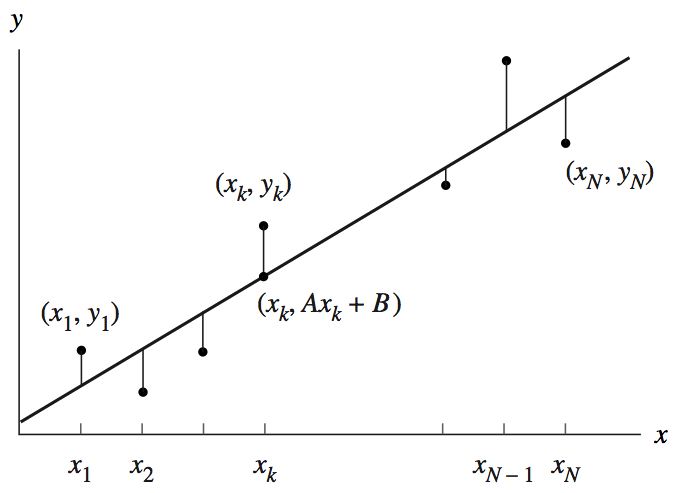
\includegraphics[width=50mm]{chap-4/fig_5-2.png}
\end{center}
\end{figure}
}

\frame{
\frametitle{Proof of Theorem }
\framesubtitle{continue 1}
\begin{itemize}
\item The minimum value of $E(A, B)$ is determined by setting the partial derivatives $ \partial E / \partial A$ and $ \partial E / \partial B$ equal to zero and solving these equations for $A$ and $B$. 
\item Notice that $\{ x_k \}$ and $\{ y_k \}$ are constants in equation (4.11) and that $A$ and $B$ are the variables! 
\item Hold $B$ fixed, differentiate $E(A, B)$ with respect to $A$, and get 
\begin{equation*}
\frac{\partial E (A, B)}{\partial A} = \sum_{k=1}^N 2 (A x_k + B - y_k) (x_k) = 2 \sum_{k=1}^N  (A x_k^2 + B x_k - x_k y_k)
\end{equation*}
\item Hold $A$ fixed and differentiate $E(A, B)$ with respect to $B$ and get 
\begin{equation*}
\frac{\partial E (A, B)}{\partial B} = \sum_{k=1}^N 2 (A x_k + B - y_k) = 2 \sum_{k=1}^N  (A x_k + B  -  y_k)
\end{equation*}
\end{itemize}
}

\frame{
\frametitle{Proof of Theorem }
\framesubtitle{continue 2}
Setting the partial derivatives equal to zero, use the distributive properties of summation to obtain
\begin{equation*}
\begin{array}{l}
\frac{\partial E (A, B)}{\partial A} = 0 \\ \\
0 = \sum_{k=1}^N  (A x_k^2 + B x_k - x_k y_k) = A \sum_{k=1}^N x_k^2 + B \sum_{k=1}^N x_k - \sum_{k=1}^N x_k y_k \\
\\ \\
\frac{\partial E (A, B)}{\partial B} = 0 \\ \\
0 = \sum_{k=1}^N  (A x_k + B  -  y_k) = A \sum_{k=1}^N x_k + NB - \sum_{k=1}^N y_k
\end{array}
\end{equation*}
}

\frame{
\frametitle{Proof of Theorem }
\framesubtitle{continue 3}
\begin{itemize}
\item the above Equations can be rearranged in the standard form for a system and result in the normal equations . 
\vspace{0.5cm}
\item The solution to this system can be obtained by one of the techniques for solving a linear system from following Chapter \footnote{ Solution of Linear Systems $AX = B$}. 
%\vspace{0.5cm}
%\item However, the method employed in Program 4.1 translates the data points so that a well-conditioned matrix is employed (see the Exercises). 
\end{itemize}
}

\frame{
\frametitle{Example }
\begin{block}{}
Find the least-squares line for the data points given in Example.
\end{block}
\begin{block}{}
The sums required for the normal equations  are easily obtained using the values in the given table . 
The linear system involving $A$ and $B$ is
\begin{equation*}
\begin{array}{l}
92 A + 20 B =25 \\
20 A + 8B = 37
\end{array}
\end{equation*}
The solution of the linear system is $A \approx −1.6071429$ and $B \approx 8.6428571$. Therefore, the least-squares line is 
\begin{equation*}
y = −1.6071429x + 8.6428571
\end{equation*}
\end{block}
}

\frame{
\begin{columns}
\begin{column}{0.5\textwidth}
\begin{figure}
\begin{center}
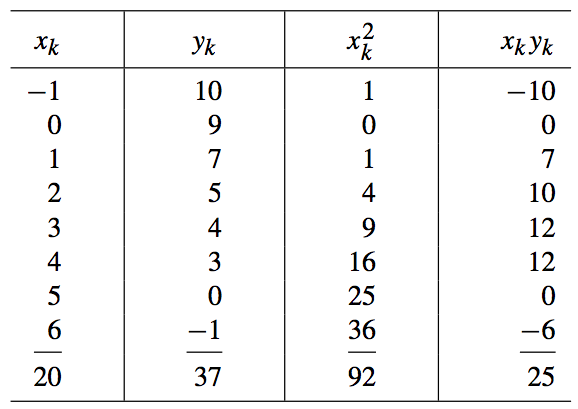
\includegraphics[width=50mm]{chap-4/tab_5-2.png}
\end{center}
\end{figure}
\end{column}
\begin{column}{0.5\textwidth}
\begin{figure}
\begin{center}
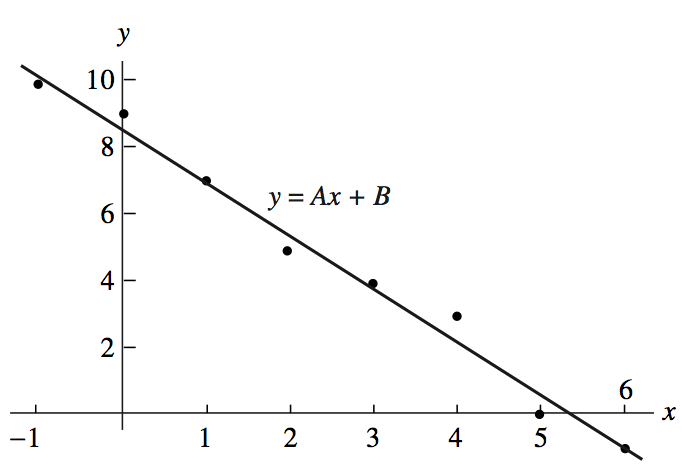
\includegraphics[width=50mm]{chap-4/fig_5-3.png}
\end{center}
\end{figure}
\end{column}
\end{columns}
}

\frame{
\frametitle{Power Fit $y=Ax^M$}
\begin{itemize}
\item Some situations involve $f(x) = Ax^M$, where $M$ is a known constant. 
\vspace{0.5cm}
\item The example of planetary motion given in Figure 4.1 is an example. 
\vspace{0.5cm}
\item In these cases there is only one parameter $A$ to be determined. 
\end{itemize}
}

\frame{
\begin{block}{Theorem (Power Fit).}
Suppose that $\{(x_k , y_k )\}^N_{k=1}$ are $N$ points, where the abscissas are distinct. 
The coefficient $A$ of the least-squares power curve $y = Ax^M$ is given by
\begin{equation*}
A = \frac{ \left( \sum_{k=1}^N x_k^M y_k \right) }{ \left(  \sum_{k=1}^N x_k^{2M}  \right) }
\end{equation*}
Using the least-squares technique, we seek a minimum of the function $E(A)$:
\begin{equation*}
E(A) = \sum_{k=1}^N \left( A x_k^M - y_k \right)^2
\end{equation*}
\end{block}
}

\frame{
\begin{block}{Theorem  (continue)}
In this case it will suffice to solve $E′(A) = 0$. The derivative is
\begin{equation*}
E′(A) = 2 \sum_{k=1}^N (A x_k^M - y_k)(x_k^M) = 2 \sum_{k=1}^N (A x_k^{2M} - x_k^M y_k)
\end{equation*}
Hence the coefficient A is the solution of the equation
\begin{equation*}
0 = A \sum_{k=1}^N x_k^{2M} - \sum_{k=1}^N x_k^My_k
\end{equation*}
\end{block}
}

\frame{
\frametitle{Example }
Students collected the experimental data in the following table . 
The relation is $d = \frac{1}{2} gt^2$, where $d$ is distance in meters and $t$ is time in seconds. 
Find the gravitational constant $g$.
\begin{figure}
\begin{center}
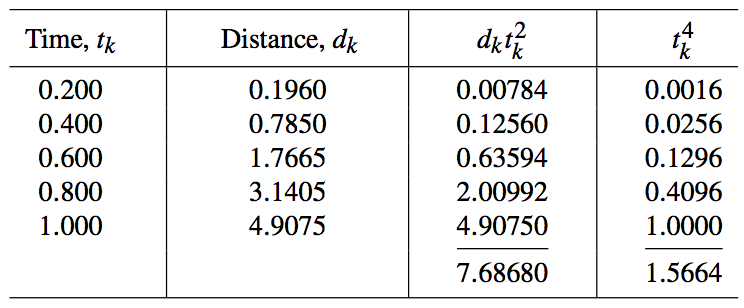
\includegraphics[width=60mm]{chap-4/tab_5-3.png}
\end{center}
\end{figure}
The values in table are used to find the summations required in formula (16),  where the power used is $M = 2$.
The coefficient is $A = 7.68680/1.5664 = 4.9073$, and we get $d = 4.9073 t^2$ and $g = 2A = 9.7146 m/sec^2$.
}


